\documentclass{article}
\usepackage{blindtext, titlesec, amsthm, thmtools, amsmath, amsfonts, scalerel, amssymb, graphicx, titlesec, xcolor, multicol, hyperref}
\usepackage[utf8]{inputenc}
\usepackage{biblatex}
% \addbibresource{./reference/reference.bib}
% For hyperlink:
\hypersetup{colorlinks, linkcolor={red!40!black}, citecolor={blue!50!black}, urlcolor={blue!80!black}}

%Latex Environment 
\newtheorem{theorem}{Theorem}[section]
\newtheorem{lemma}[theorem]{Lemma}
\newtheorem{corollary}{Corollarium}[section]
\theoremstyle{definition}
\newtheorem{definition}{Definition}[section]
\newtheorem{proposition}{Proposition}[definition]

\theoremstyle{definition}
\newtheorem{axiom}{Axiom}[section]

\theoremstyle{remark}
\newtheorem{remark}{Observatio}[section]
\newtheorem{hypothesis}{Coniectura}[section]
\newtheorem{example}{Exampli Gratia}[section]

% Renew Command 
\renewenvironment{proof}{{\emph{Demonstratio.}}}{\qed}
% \renewenvironment{proof}{{\bfseries\emph{Demonstratio.}}}{\qed}
\renewcommand\qedsymbol{Q.E.D.}

\graphicspath{{images/}}
\usepackage{amssymb}

\title{Proofs and Problem Solving}
\author{Li Qianrui}

\begin{document}

\maketitle
\tableofcontents

\newpage

\section{Upper bounds and Least upper bound}

\subsection{Upper and Lower Bounds}
%Definition 5.1: Let A be a subset of R \\

\begin{figure}[h]
    \centering
    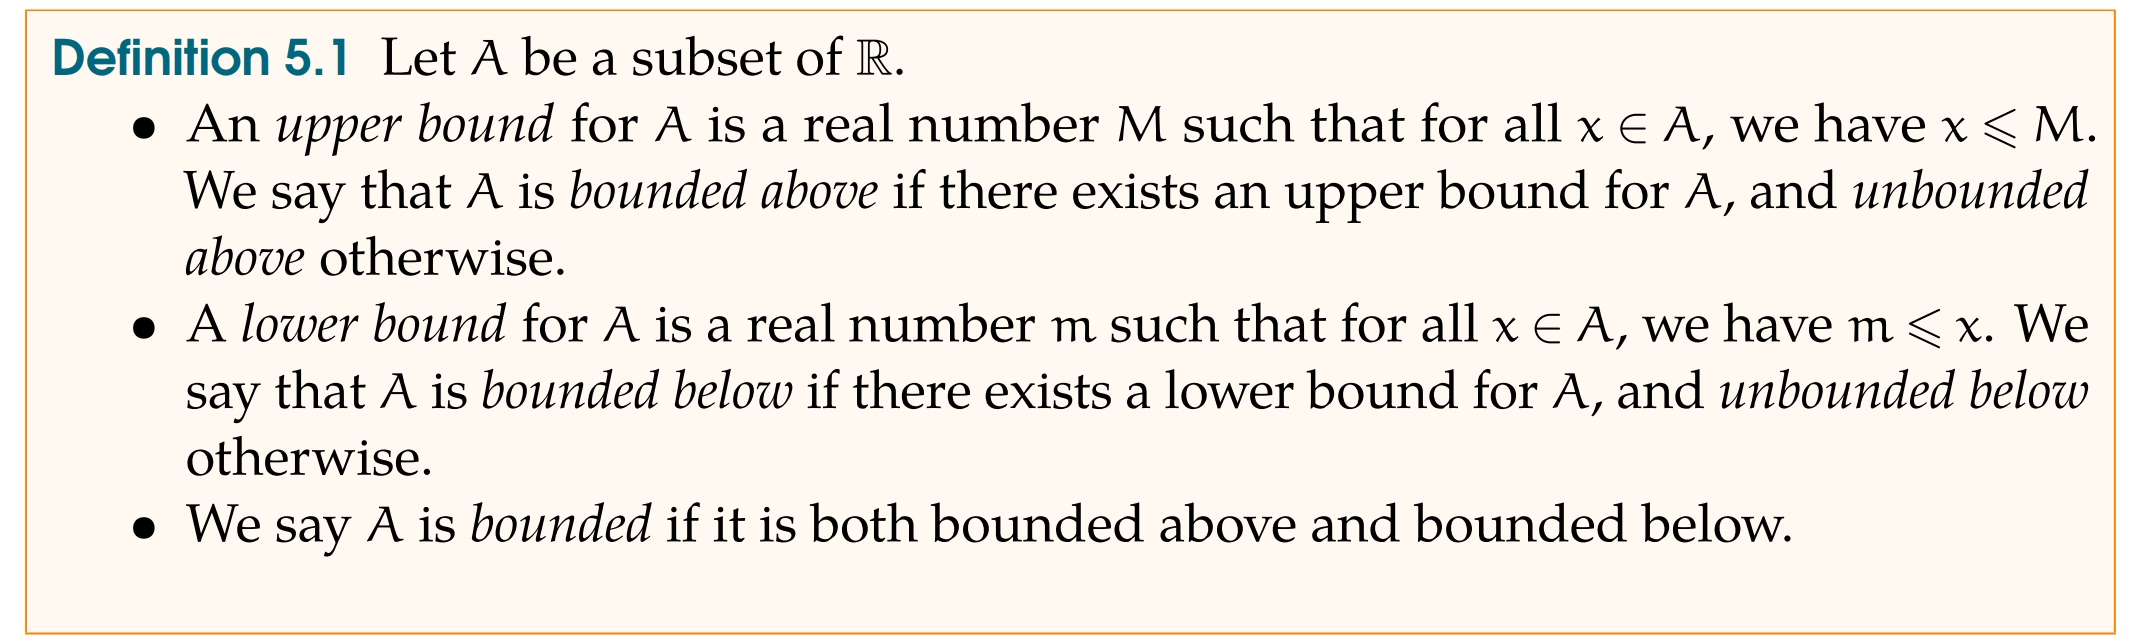
\includegraphics[width=0.9\textwidth]{Definition5.1}\\
    %\caption{A nice plot.}
    %\label{fig:mesh1}
\end{figure}

\subsection{Least Upper Bounds and Greatest Lower Bounds}

\begin{definition}[Least Upper Bound]
Given a subset $A\subseteq \mathbb{R}$, a number L is a \textbf{least upper bound (LUB)} or supremum for A if and only if:
\begin{enumerate}
	\item L is an upper bound for A, that is, $x\leq L$ for all $x\in A$;\\
	% TODO Need Rephrasing.
	\item $L\leq M$ for every upper bound M of A \textbf{or} \\ for all $t < L$, there exist $x\in A$ such that $x>t$.\\
\end{enumerate}
This is definition 5.2 in the textbook.
\end{definition}

\begin{definition}[Greatest Lower Bound]
\end{definition}

\subsection{Completeness Axiom for the real numbers}
Every nonempty subset of $\mathbb{R}$ that is bounded above has a \emph{least upper bound}.\\

\begin{theorem}[The Archimedean Property]
For any $x,y\in \mathbb{R}$ with $x,y>0$, there is some $n\in \mathbb{N}$ such that $ny>x$. (Theorem 5.1 in the textbook).
\end{theorem}
\begin{remark}
Could be prove by contradiction
\end{remark}

\newpage

\section {Limits}

\subsection{The $\epsilon-\mathbb{N}$ definition of a limit.}
Let ${(x_{n})}{_{n=1}^{\infty}}$ be a sequence of real numbers x1,x2,... and let $L\in \mathbb{R}$. We say that $x_{n}$ \textbf{converge} to L, or L us the \textbf{limit} of the sequence $(x_{n})$,if for all $\epsilon > 0$, there exists a natural numebr N such that for all $n>N$,\\

\begin{center}

$|x_{n}-L| < \epsilon$,\\

\end{center}


When $x_{n}$ converges to L, we write $x_{n} \rightarrow L$ as $n\rightarrow \infty$, or $\lim_{n\rightarrow \infty}x_{n}=L$.

\subsection{Bounded Sequence}

\begin{definition}
    We say that a sequence $(a_{n})$ is \textbf{bounded} if the set of values {a1,a2,...} is a bounded set. 
    i.e. there are m,M such that $m \leq a_{n} \leq M$ for all n.
\end{definition}

\begin{proposition}
    Suppose the sequence $(a_{n})$ converges. Then it is bounded.
\end{proposition}

\begin{proposition}
    Suppose that $x_{n} \rightarrow L$ as $n \rightarrow \infty$ and that $k \in \mathbb{N}$. Then $x{_{n}^{k}} \rightarrow L^{k}$ as $n \rightarrow \infty$.\\
\end{proposition}

\subsection {Application: the existence of roots}
\textbf{Theorem 6.6}\\
Let $x>0$ and $k \in \mathbb{N}$. Then there is a unique $y>0$ such that $y^{k}=x$.\\

\subsection {Infinite limits}
\textbf{Definition 6.4}
Let ${x_{n}}$ be a sequence of real numbers.\\
\\
(a) We say $(x_{n})$ tends to $\infty$ or \textbf{diverges} to $\infty$, and write $x_{n}\rightarrow \infty$ as $n \rightarrow \infty$ if for all $M > 0$, there exists $N \in \mathbb{N}$ such that $n>N$ implies $x_{n}\geq M$.\\
\\
(b) Similar for $x_{n} \rightarrow -\infty$
\pagebreak


\section{The monotone Convergence Theorem}
\subsection{Monotonic}
A sequence $(a_{n}){_{n=1}^{\infty}}$ is \textbf{increasing} if $a_{n+1} \geq a_{n} $ for all n. It is \textbf{decreasing} if $a_{n+1}\leq a_{n}$ for all n. We say ${a_n}$ is \textbf{monotonic} if it is either increasing or decreasing. \\
\\
\textbf{Monotone Convergence Theorem (MCT)}\\
Let $(a_{n})$ be an \textbf{increasing} sequence of real numbers that is bounded above (i.e. there is M so that $a_{n}\leq M$ for all n). Then $(a_{n})$ converges to some limit.\\
Similar to \textbf{decreasing} sequence. \\

\subsection{literatively defined sequence}
The value of $x_{n+1}$ is specified in terms of previous values of the sequence $x_{1}, ..., x_{n}$, (usually $x_{n}$).
\pagebreak


\section{Decimals and Series}
Every real number has a decinal expansion, and conversely, every decimal expansion gives rise to a real number.

\subsection{Decimals}
\textbf{Theorem 8.1}\\
Given sequence $(a_{n})$ with $a_{n} \in {0,1,...,9}$ for all n, the decimal expanision $x=0.a_{1}a_{2}a_{3}a_{4}...a_{n}...$ given by the limit of the sequence \\

\begin{equation}
    x_{n}=\frac{a_{1}}{10}+\frac{{a}_{2}}{100}+...+\frac{{a}_{n}}{10^{n}}
\end{equation}


defines a real number x satisfying $0 \leq x \leq 1$.\\
\\
\textbf{Theorem 8.3}\\
Let $0\leq x \leq 1$ and suppose that $x=0.{a}_{1}{a}_{2}... = 0.{b}_{1}{b}_{2}...$. Let \textit{l} be the smallest integer for which ${a}_{\textit{l}} \neq {b}_{\textit{l}}$ and suppose that ${a}_{\textit{l}} < {b}_{\textit{l}}$.
Then ${b}_{\textit{l}} = {a}_{\textit{l}}+1$, and for all $k > \textit{l}$ we have ${b}_{\textit{k}}=0$ and ${a}_{\textit{l}}=9$.

\textbf{Corollary 8.5 - of the proof.}\\
If \textit{p} and \textit{q} are positive inegers, the rational number \textit{p}/\textit{q}
has a decimal expansion with period at most \textit{q}.\\
\\
\textbf{Theorem 8.7}\\
A number $x \geq 0$ is ration $\Leftrightarrow$ it has periodic decimal expansion. \\
\\
\textbf{Corollary 8.8}\\
A number $x \geq 0$ is irrational $\Leftrightarrow$ if has aperiodic decimal expansion\\
\\
\textbf{Definition 8.2}\\
Given a sequence ${{a}_{j}}$, we say that the infinite series ${\sum{^{\infty}_{j=1}}{a}_{j}}$ \emph{converges} if 
the sequence of partial sums \\
\begin{equation}
    {s}_{n}={\sum{^{n}_{j=1}}{a}_{j}}
\end{equation}
converges as $n \rightarrow \infty$. When (${s}_{n}$) converges we denote its limit by ${\sum{^{\infty}_{j=1}}{a}_{j}}$.\\

\subsection{The number e}
\begin{equation}
    e: = {\sum{^{\infty}_{n=0}}\frac{1}{n!}} = \lim_{n \rightarrow \infty}(1+\frac{1}{n})^{n}
\end{equation}

\newpage

\section{Complex number}
\subsection{Definition 9.1 - Complex numbers definition}
Define i to be a number such that $i^2 = -1$ \\
The \textbf{comple numbers} are any number of the form 
\begin{equation}
    z=x+iy where x,y \in \mathbb{R}
\end{equation}
The set of all complex numbers is denoted $\mathbb{C}$\\
We define Re(z)=x and Im(z)=y to be the \textbf{real} and \textbf{imaginary} parts of z.\\

\subsection{Argand diagram}
\begin{center}
    \centering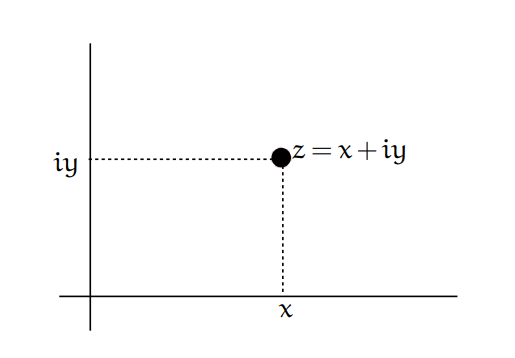
\includegraphics[scale = 0.6]{Graph 9.0}\\
\end{center}



\subsection{Definition 9.2 - Modulus}
\begin{center}
    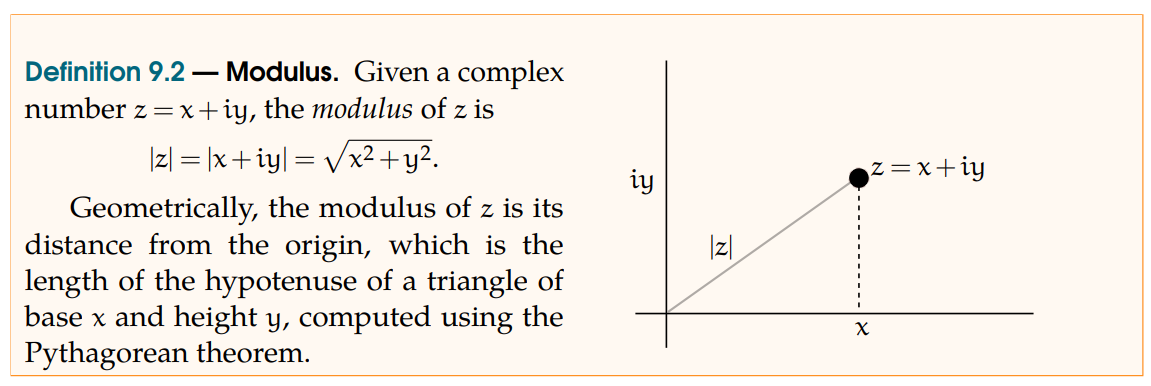
\includegraphics[width=0.9\textwidth]{Definition 9.2}\\
\end{center}


\subsection{Definition 9.3 - Complex conjugate}
\begin{center}
    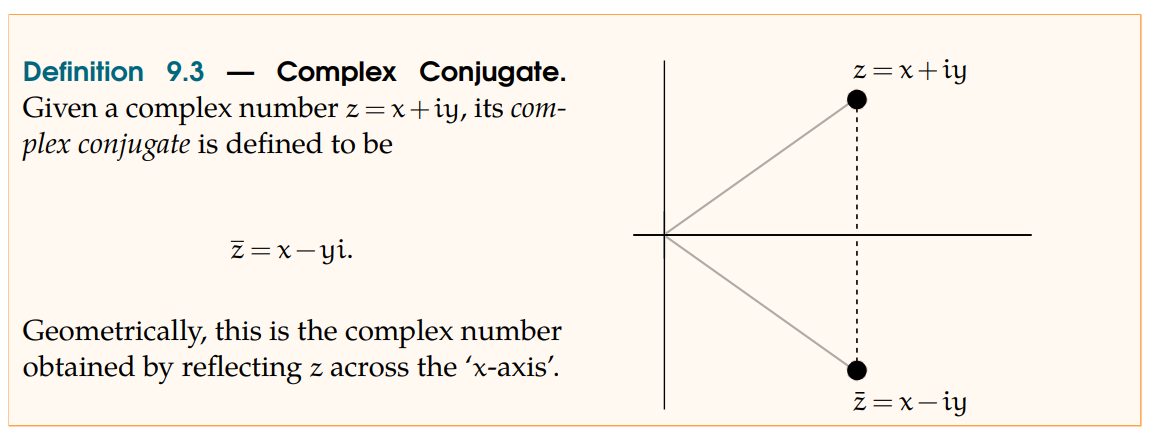
\includegraphics[width=0.9\textwidth]{Definition 9.3}\\
\end{center}


\subsection{Definition 9.4 - Cartesian and Polar form}
\begin{center}
    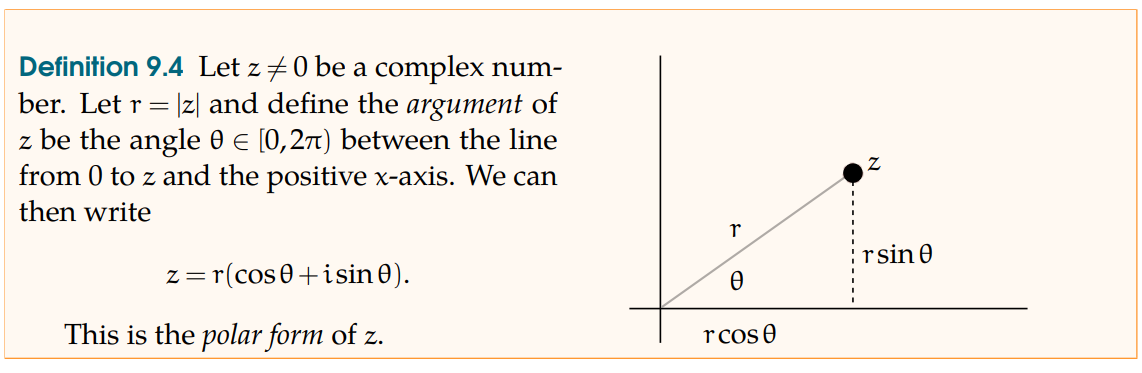
\includegraphics[width=0.9\textwidth]{Definition 9.4}\\
\end{center}

\subsection{multiplication of complex}
Let $z=r(cos \theta +isin \theta)$ and  $w=s(cos \phi + isin\phi)$\\
\begin{equation} 
\begin{aligned}
    zw = r(cos \theta + isin\theta)\times s(cos\phi + isin\phi)\\
    = rs(cos(\theta + \phi)+isin(\theta + \phi))
\end{aligned}
\end{equation}
\\
\textbf{De Movivre's Theorem}\\
If we let $z=r(cos\theta + isin\theta)$, and $n\in \mathbb{N}$, then\\
\begin{equation}
\begin{aligned}
    z^n = r^n(cos n\theta + isin n\theta)\\
    z^{-n} = r^{-n}(cos(-n\theta)+ isin(-n \theta)) = \frac{1}{r^{n}}(cos(n \theta)-isin(n\theta))
\end{aligned}
\end{equation}
\\

\subsection{Exponential form: Euler's formula}
\begin{center}
\begin{equation}
    e^{i \theta} = cos(\theta)+isin(\theta)
\end{equation}
\end{center}

\textbf{Special case 1:}\\
\begin{center}
    $e^{i \pi} = -1$
\end{center}

\textbf{Special case 2:}\\
\begin{center}
    $z=re^{i\theta}= r(cos\theta + isin\theta)$
\end{center}

\subsection{Theorem9.4 - Roots of Unity}
The solutions to $z^n = 1$ are $1,w,...w^{n-1}$ where $w=e^{\frac{2\pi i}{n}}$, 
That is, they are $e^{\frac{2\pi k i}{n}}$ for k=0,1,..., n-1.

\newpage
\section{Polynomials}
\subsection{Definition 10.1}
For $n\in \mathbb{N}$, and n-degree complex polynomial \emph{p} is a 
function of the form

\begin{equation}
    p(z)={a}_{n}z^{n} + {a}_{n-1}z^{n-1}+ ... + {a}_{0}
\end{equation}


where ${a}_{n} \neq 0$ and ${a}_{i} \in \mathbb{C}$ for all i.\\
    n is called the \emph{degree} of the polynomial \\
    A \emph{root} of p is a complex number $\alpha \in \mathbb{C}$ 
    such that $p(\alpha) = 0$.\\

\subsection{Abel-Ruffini Theorem}
There is no formula for the roots of a polynomial of degree $\geq$ 5.\\

\subsection{Theorem 10.2 - Fundamental Theorem of Algebra.}
Any complex polynomial has at least one root in $\mathbb{C}$.\\

\subsection{Theorem 10.3 - Factorization Theorem}
If p is a degree n polynomial, then there are n roots ${r}_{1},...,{r}_{n} \in \mathbb{C}$ 
and a number $a \in \mathbb{C}$ so that 
\begin{equation}
    p(z)=a(z-{r}_{1})(z-{r}_{2})...(z-{r}_{n}).
\end{equation}

\subsection{Theorem 10.4 - Real Polynomials}
Real Polynomials have \emph{conjugated roots}. \\
If p(x) has real coefficients and r is a root, so is $\bar(r)$.


\subsection{Theorem 10.5 - Root-Coefficient Theorem} 
If $ p(x) = x^n +{a}_{n-1}x^{n-1}+ ... + {a}_{1}x+{a}_{0}$, has roots ${r}_{1},...,{r}_{n}$ (counting multiplicities), 
then
\begin{equation}
\begin{aligned}
    {r}_{1}+ ... +{r}_{n} = -{a}_{n-1}
    {r}_{1}...{r}_{n} = (-1)^{a}_{0}
\end{aligned}
\end{equation}

In general, if ${s}_{j}$ denotes the sum of all products of j-tuples of the roots 
(e.g. ${s}_{2} = {r}_{1}{r}_{2}+{r}_{1}{r}_{3}+{r}_{2}{r}_{3}+...$), then\\
\begin{equation}
    {s}_{j}=(-1)^j {a}_{n-j}.
\end{equation}







\end{document}
